
%使用XeLaTeX编译
%版权所有,翻版必究
%本文件由程序自动生成,任何修改将被覆盖
%2019 年 01 月 23 日




\FloatBarrier
\section{
Blend
}\label{c000015s000002}


Blend特效常用属性
如\tablename\ \ref{tb000001}:


%使用XeLaTeX编译
%版权所有,翻版必究
%本文件由程序自动生成,任何修改将被覆盖
%2019 年 01 月 23 日



%表
\begin{longtable}{ccc}

%表头....
\toprule{}类名 
&
分类
&
简介%there must use marginnote ...
\marginnote{\setlength\fboxsep{2pt}\fbox{\footnotesize{\kaishu\tablename\,}\footnotesize{\ref{tb000000}}}}
\\ \midrule 
\endfirsthead

%表尾...
\bottomrule
\caption{ThresholdMask}\label{tb000000} 
\endlastfoot

%重复表头
\toprule{}类名 
&
分类
&
简介
\\ \midrule
\endhead
%重复表尾
\midrule
\endfoot 
Blend & aabbc & cccc \\
BrightnessContrast & aabbc & cccc \\
ColorOverlay & aabbc & cccc \\
Colorize & aabbc & cccc \\
Desaturate & aabbc & cccc \\
GammaAdjust & aabbc & cccc \\
HueSaturation & aabbc & cccc \\
LevelAdjust & aabbc & cccc \\
ConicalGradient & aabbc & cccc \\
LinearGradient & aabbc & cccc \\
RadialGradient & aabbc & cccc \\
Displace & aabbc & cccc \\
DropShadow & aabbc & cccc \\
InnerShadow & aabbc & cccc \\
FastBlur & aabbc & cccc \\
GaussianBlur & aabbc & cccc \\
MaskedBlur & aabbc & cccc \\
RecursiveBlur & aabbc & cccc \\
DirectionalBlur & aabbc & cccc \\
RadialBlur & aabbc & cccc \\
ZoomBlur & aabbc & cccc \\
Glow & aabbc & cccc \\
RectangularGlow & aabbc & cccc \\
OpacityMask & aabbc & cccc \\
ThresholdMask  & aabbc & cccc \\
\end{longtable}
%表





%使用XeLaTeX编译
%版权所有,翻版必究
%本文件由程序自动生成,任何修改将被覆盖
%2019 年 01 月 23 日





混合类型
如\tablename\ \ref{tb000002}
    \footnote{对于图片处理中常见术语,本书不赘述。}
:


%使用XeLaTeX编译
%版权所有,翻版必究
%本文件由程序自动生成,任何修改将被覆盖
%2019 年 01 月 23 日



%表
\begin{longtable}{ccc}

%表头....
\toprule{}类名 
&
分类
&
简介%there must use marginnote ...
\marginnote{\setlength\fboxsep{2pt}\fbox{\footnotesize{\kaishu\tablename\,}\footnotesize{\ref{tb000000}}}}
\\ \midrule 
\endfirsthead

%表尾...
\bottomrule
\caption{ThresholdMask}\label{tb000000} 
\endlastfoot

%重复表头
\toprule{}类名 
&
分类
&
简介
\\ \midrule
\endhead
%重复表尾
\midrule
\endfoot 
Blend & aabbc & cccc \\
BrightnessContrast & aabbc & cccc \\
ColorOverlay & aabbc & cccc \\
Colorize & aabbc & cccc \\
Desaturate & aabbc & cccc \\
GammaAdjust & aabbc & cccc \\
HueSaturation & aabbc & cccc \\
LevelAdjust & aabbc & cccc \\
ConicalGradient & aabbc & cccc \\
LinearGradient & aabbc & cccc \\
RadialGradient & aabbc & cccc \\
Displace & aabbc & cccc \\
DropShadow & aabbc & cccc \\
InnerShadow & aabbc & cccc \\
FastBlur & aabbc & cccc \\
GaussianBlur & aabbc & cccc \\
MaskedBlur & aabbc & cccc \\
RecursiveBlur & aabbc & cccc \\
DirectionalBlur & aabbc & cccc \\
RadialBlur & aabbc & cccc \\
ZoomBlur & aabbc & cccc \\
Glow & aabbc & cccc \\
RectangularGlow & aabbc & cccc \\
OpacityMask & aabbc & cccc \\
ThresholdMask  & aabbc & cccc \\
\end{longtable}
%表





%使用XeLaTeX编译
%版权所有,翻版必究
%本文件由程序自动生成,任何修改将被覆盖
%2019 年 01 月 23 日





%begin图片
\begin{figure}[htb] %浮动体 here and top ...
%there must use marginnote ...
\marginnote{\setlength\fboxsep{2pt}\fbox{\footnotesize{\kaishu\figurename\,}\footnotesize{\ref{p000018}}}}\centering %中心对齐
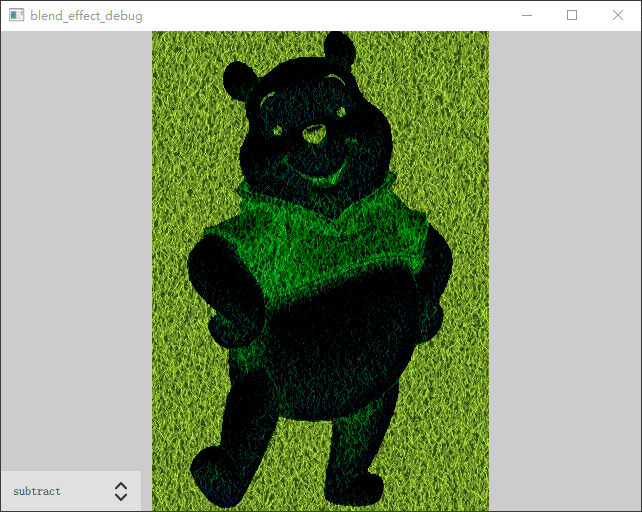
\includegraphics[width=0.95\textwidth]{../chapter06/blend_effect/the_app.png} %图片路径
\caption{Blend} %标题
\label{p000018} %索引
\end{figure}
%end图片


%\begin{spacing}{1.0}
\refstepcounter{filesourcenumber}\label{f000052}    %增加源代码编号
\FloatBarrier                                  %强制完成浮动体布局
\begin{thebookfilesourceone}[escapeinside={(*@}{@*)},
caption=GoodLuck,
title=\filesourcenumbernameone \thefilesourcenumber
]
/*blend_effect/main.qml*/
import QtQuick 2.9
import QtGraphicalEffects 1.12

Rectangle {
    id : idRoot
    width: 640;
    height: 480;
    color: Qt.rgba(0.8,0.8,0.8,1);

    Image{
        anchors.fill: parent;
        source: "grass.jpg"
        fillMode: Image.Tile
        id : idGrass
        visible: false
    }

    Image{
        anchors.centerIn: parent;
        source: "bear.png"
        fillMode: Image.Stretch
        id : idBear
        visible: false
    }

    Blend{
        source: idGrass
        foregroundSource: idBear
        mode: idBlendControl.blendModeComboBox.currentText
        anchors.centerIn: parent;
        width: idBear.width
        height: idBear.height
    }

    BlendControl {
        id : idBlendControl
    }

}(*@\marginpar[\hfill\setlength\fboxsep{2pt}\fbox{\footnotesize{\kaishu\parbox{1em}{\setlength{\baselineskip}{2pt}\filesourcenumbernameone}}\footnotesize{\thefilesourcenumber}}]{\setlength\fboxsep{2pt}\fbox{\footnotesize{\kaishu\parbox{1em}{\setlength{\baselineskip}{2pt}\filesourcenumbernameone}}\footnotesize{\thefilesourcenumber}}}@*)\end{thebookfilesourceone}          %抄录环境
\addtocounter{lstlisting}{-1}   %sub lstlisting counter ...
%\end{spacing}


 






%使用XeLaTeX编译
%版权所有,翻版必究
%本文件由程序自动生成,任何修改将被覆盖
%2019 年 01 月 23 日



